%latex model.tex
%bibtex model
%latex model.tex
%latex model.tex
%pdflatex model.tex

%se poate lucra si online (de ex www.overleaf.com)


\documentclass[runningheads,a4paper,11pt]{report}

\usepackage{algorithmic}
\usepackage{algorithm} 
\usepackage{array}
\usepackage{amsmath}
\usepackage{amsfonts}
\usepackage{amssymb}
\usepackage{amsthm}
\usepackage{caption}
\usepackage{comment} 
\usepackage{epsfig} 
\usepackage{fancyhdr}
\usepackage[T1]{fontenc}
\usepackage{geometry} 
\usepackage{graphicx}
\usepackage[colorlinks]{hyperref} 
\usepackage[latin1]{inputenc}
\usepackage{multicol}
\usepackage{multirow} 
\usepackage{rotating}
\usepackage{setspace}
\usepackage{subfigure}
\usepackage{url}
\usepackage{verbatim}
\usepackage{xcolor}
\usepackage{float}

\geometry{a4paper,top=3cm,left=2cm,right=2cm,bottom=3cm}

\pagestyle{fancy}
\fancyhf{}
\fancyhead[LE,RO]{Estimation of Land Surface Temperature}
\fancyhead[RE,LO]{Satellite Scalers}
\fancyfoot[RE,LO]{MIRPR 2024-2025}
\fancyfoot[LE,RO]{\thepage}

\renewcommand{\headrulewidth}{2pt}
\renewcommand{\footrulewidth}{1pt}
\renewcommand{\headrule}{\hbox to\headwidth{%
  \color{lime}\leaders\hrule height \headrulewidth\hfill}}
\renewcommand{\footrule}{\hbox to\headwidth{%
  \color{lime}\leaders\hrule height \footrulewidth\hfill}}

\hypersetup{
pdftitle={artTitle},
pdfauthor={name},
pdfkeywords={pdf, latex, tex, ps2pdf, dvipdfm, pdflatex},
bookmarksnumbered,
pdfstartview={FitH},
urlcolor=cyan,
colorlinks=true,
linkcolor=red,
citecolor=green,
}
% \pagestyle{plain}

\setcounter{secnumdepth}{3}
\setcounter{tocdepth}{3}

\linespread{1}

% \pagestyle{myheadings}

\makeindex


\begin{document}

\begin{titlepage}
\sloppy

\begin{center}
BABE\c S BOLYAI UNIVERSITY, CLUJ NAPOCA, ROM\^ ANIA

FACULTY OF MATHEMATICS AND COMPUTER SCIENCE

\vspace{6cm}

\Huge \textbf{Estimation of Land Surface Temperature}

\vspace{1cm}

\normalsize -- MIRPR report --

\end{center}


\vspace{5cm}

\begin{flushright}
\Large{\textbf{Team members}}\\
Vaida Bogdan, IR, Gr. 237, bogdan.alexandru.vaida@stud.ubbcluj.ro\\
Voina Marius, IR, Gr. 237, marius.voina@stud.ubbcluj.ro

\end{flushright}

\vspace{4cm}

\begin{center}
2024-2025
\end{center}

\end{titlepage}

\pagenumbering{gobble}

\begin{abstract}
Estimating street-level air temperatures in urban environments is no easy feat. The varied nature of urban surfaces, the canyon-like streets, and the myriad physical processes at play make this a challenging task. In this project, we dive into the world of Graph Neural Networks (GNN) and spatial embeddings to boost the resolution of satellite images. Our aim? To enhance urban planning and policies by making cities more resilient to climate change, paving the way for better environmental management and sustainability. The magic ingredients in our approach are GNN and embeddings. We've worked with satellite images of different resolutions, and the results? A significant leap in the accuracy of street-level temperature estimations.
\end{abstract}

\begin{figure}[H]
\centering
\includegraphics[width=0.8\textwidth]{GNN_process.png}
\caption{Overview of the GNN process for enhancing satellite image resolution}
\label{fig:GNN_process}
\end{figure}


\tableofcontents

\newpage

\listoftables
\listoffigures
\listofalgorithms

\newpage

\setstretch{1.5}



\newpage

\pagenumbering{arabic}


 


\chapter{Introduction}\label{chapter:introduction}
\section{What? Why? How?}\label{section:what}

Graph Neural Networks (GNN) are a type of neural network designed to operate on graph structures. Unlike traditional neural networks, which process data in a fixed format, GNNs excel in capturing the relationships and dependencies between nodes in a graph. This makes them particularly suitable for spatial data, where the context and connectivity between different locations are crucial.

In this project, GNNs are employed to enhance the resolution of satellite images, making it possible to generate high-resolution temperature maps from lower-resolution data. By integrating these advanced techniques, the project aims to contribute significantly to urban planning and policy, promoting environmental management and urban sustainability, and ultimately enhancing the resilience of cities to climate change.

\section{Paper structure and original contribution(s)}\label{section:structure}
This project represents the journey of exploring the potential of Graph Neural Networks (GNN) to tackle the challenging problem of estimating land surface temperatures in urban settings. Our primary contribution lies in the development of an intelligent algorithm that leverages GNN and spatial embeddings to significantly enhance the resolution of satellite images.

This report is structured to take you through our process, insights, and findings, broken down into 
\begin{itemize}
    \item The first chapter is a short introduction.
    \item The second chapter describes the scientific problem.
    \item The third chapter details the related work and useful tools.
    \item The fourth chapter outlines the proposed approach.
    \item The fifth chapter presents the application and results.
\end{itemize}



\chapter{Scientific Problem}
\label{section:scientificProblem}

\section{Problem Definition}
\label{section:problemDefinition}

Estimating land surface temperatures (LST) at street level in urban areas is no stroll in the park. Urban environments are like intricate puzzles, with their complex surfaces, canyon-like streets, and the myriad physical processes at play. This complexity makes it essential to find innovative solutions to accurately estimate temperatures for better urban planning and to bolster climate resilience.\\
Enter the world of GNNs and spatial embeddings. These powerful tools allow us to harness satellite images of various resolutions and transform them into high-accuracy temperature maps. By applying GNNs, which are adept at understanding the relationships and dependencies between different nodes (or locations) in a graph, we can significantly improve the resolution and accuracy of LST estimates.




\chapter{State of the Art / Related Work}\label{chapter:stateOfArt}

The quest to accurately estimate urban temperatures has evolved significantly over the years. From traditional methods relying on ground-based observations to sophisticated machine learning techniques, the journey has been marked by various innovative approaches.

Several studies have paved the way for the application of these advanced techniques in urban climate research:

\begin{itemize}
    \item \textbf{Kim et al. (2022)}: Kim and colleagues utilized Google Street View images combined with deep learning to estimate mean radiant temperature in urban canyons. Their approach involved image segmentation and deep learning algorithms to calculate view factors and project panoramas into fisheye images, achieving a high correlation with measurement data \cite{Kim2022}.
    \item \textbf{Mitraka et al. (2015)}: Mitraka and her team proposed a spatial-spectral unmixing technique to enhance the spatial resolution of thermal infrared observations for land surface temperature (LST) estimation. Applied to an urban area in Crete, Greece, this method demonstrated a root mean square error (RMSE) of less than 2 K, showcasing its potential for improving urban temperature maps \cite{Mitraka2015}.
    \item \textbf{Li and Sharma (2024)}: Li and Sharma developed a comprehensive modeling framework using machine learning to predict street-level air temperatures from urban climate informatics. Implemented in Chicago, their framework leveraged high-resolution urban geospatial datasets and weather observations from a dense sensor network, demonstrating the practical applicability of these advanced techniques \cite{LiSharma2024}.
\end{itemize}



Graph Neural Networks (GNN) represent a significant leap forward in this domain. Unlike conventional neural networks, GNNs excel in handling graph-structured data, making them ideal for modeling spatial relationships in urban environments. By using nodes to represent different locations and edges to capture the relationships between them, GNNs can effectively estimate temperatures across varied urban landscapes.

Spatial embeddings further enhance this capability by encoding the geographical and physical properties of different locations. These embeddings allow the model to understand the intricate patterns and dependencies in the data, leading to more accurate temperature predictions. Together, GNN and spatial embeddings offer a powerful toolkit for urban temperature estimation.

The advancements in estimating temperatures highlight the promising potential of integrating machine learning and deep learning techniques, particularly GNN and spatial embeddings. These methods not only improve accuracy but also provide scalable solutions for urban climate studies. As we continue to innovate, the challenge remains to further refine these models and integrate them into practical applications for urban planning and policy-making.


\chapter{Investigated approach}
\label{chapter:proposedApproach}

\section{Dataset}

    For this project, we utilized Landsat 8 images specifically focusing on Band 10, which provides thermal infrared data. These images have a resolution of 30 meters per pixel. The data was sourced from EarthExplorer \cite{usgs}, a powerful tool for acquiring satellite imagery and other geospatial data. Band 10 captures the temperature information crucial for estimating land surface temperature.

\begin{figure}[H]
    \centering 
    \includegraphics[width=\linewidth]{example_image.png}
    \caption{Example of Landsat 8 Band 10 Image}
    \label{fig:exampleImage}
\end{figure}

\section{Data Processing} The raw Landsat 8 images were preprocessed to extract meaningful features: \begin{itemize}
    \item \textbf{Rotation and Cropping:} Each image was rotated based on the first non-zero pixel detected to align it properly, because Landsat 8 images are rotated at an angle between 12 and 14 degrees clockwise depending on the location of the image.
    \item \textbf{Normalization:} Temperature values were computed using the calibration constants for B10 (ML, AL, K1, K2). These constants are universal for every Band 10 picture, and computing them results the temperature of each individual pixel, in Kelvin.
    \item \textbf{Cropping:} Images were cropped to a fixed size (6000x6000 pixels) to maintain consistency for training and easier downsampling.
    \item \textbf{Downsampling:} The high-resolution images were downsampled to create lower-resolution inputs for training. The downsized size is 2000x2000 pixels, we take the average of 9 pixels and store it as one for the downsampled photo.
\end{itemize}

\begin{figure}[H]
    \centering
    \begin{equation}
    \text{Temperature} = \frac{K2}{\ln\left(\frac{K1}{ML \times \text{DN} + AL} + 1\right)} \end{equation}
    \caption{Formula to calculate temperature from Band 10 constants \cite{usgs2019}}
    \label{fig:tempFormula}
\end{figure}

\section{Graph Neural Network (GNN)}
We implemented a Graph Convolutional Network (GCN) model to super-resolve the downsampled images back to high-resolution predictions:

\subsection{Architecture}
The GCN model consists of three convolutional layers: 
\begin{itemize} 
    \item \textbf{Input Features:} Each pixel (node) has three features: temperature value and two positional encodings (x and y coordinates). 
    \item \textbf{Hidden Layers:} The first two GCN layers transform the input features into higher-dimensional representations. 
    \item \textbf{Output Layer:} The final GCN layer produces the output with 9 channels, representing the high-resolution pixel predictions. 
\end{itemize}

\subsection{Node and Edge Formation}
\begin{itemize}

    \item \textbf{Node Formation:} Each pixel in the low-resolution image acts as a node in the graph, with features including temperature value and position encoding
    . \item \textbf{Edge Formation:} An 8-neighborhood connectivity was established, connecting each pixel to its adjacent pixels.
    
\end{itemize}

\section{Training} The model was trained using a dataset of input-output pairs:
\begin{itemize}
    \item \textbf{Input:} The downsampled images (2000x2000 pixels) 
    \item \textbf{Output:} The original high resolution images (6000x6000 pixels)
    
    
\end{itemize}
For this we used 50 images (split 80/20) for training and validation. The training lasted for 15 epochs, using a learning rate of 0.02. 
\begin{figure}[H]
    \centering
    \includegraphics[width=\linewidth]{training_loss.png}
    \caption{Training Loss Over Time}
    \label{fig:trainingLoss}
\end{figure}

The lowest loss value that we achieved during training was 0.0017.


We tried to optimizing memory as much as possible, using a GC for RAM and flushing the cuda VRAM often. We ran into a lot of VRAM limitations, so we needed to reduce the number of hidden channels in all the convolution layers.


\section{Evaluation} The model was evaluated with the remaining images from the data split, and the following metrics were recorded:
\begin{itemize} 
    \item \textbf{Mean Squared Error (MSE):} 0.0417671762406826
    \item \textbf{Mean Absolute Error (MAE):} 0.0042164814658463 
    \item \textbf{R-squared (R2):} 0.8399149179458618
\end{itemize}

This evaluation is based on the normalized data values (between 0 and 1).

\subsection{Comparison of Images}
To visually illustrate the effectiveness of our GCN model, we include a comparison of the low-resolution image and the upscaled image predicted by the model
\begin{figure}[H]
    \centering 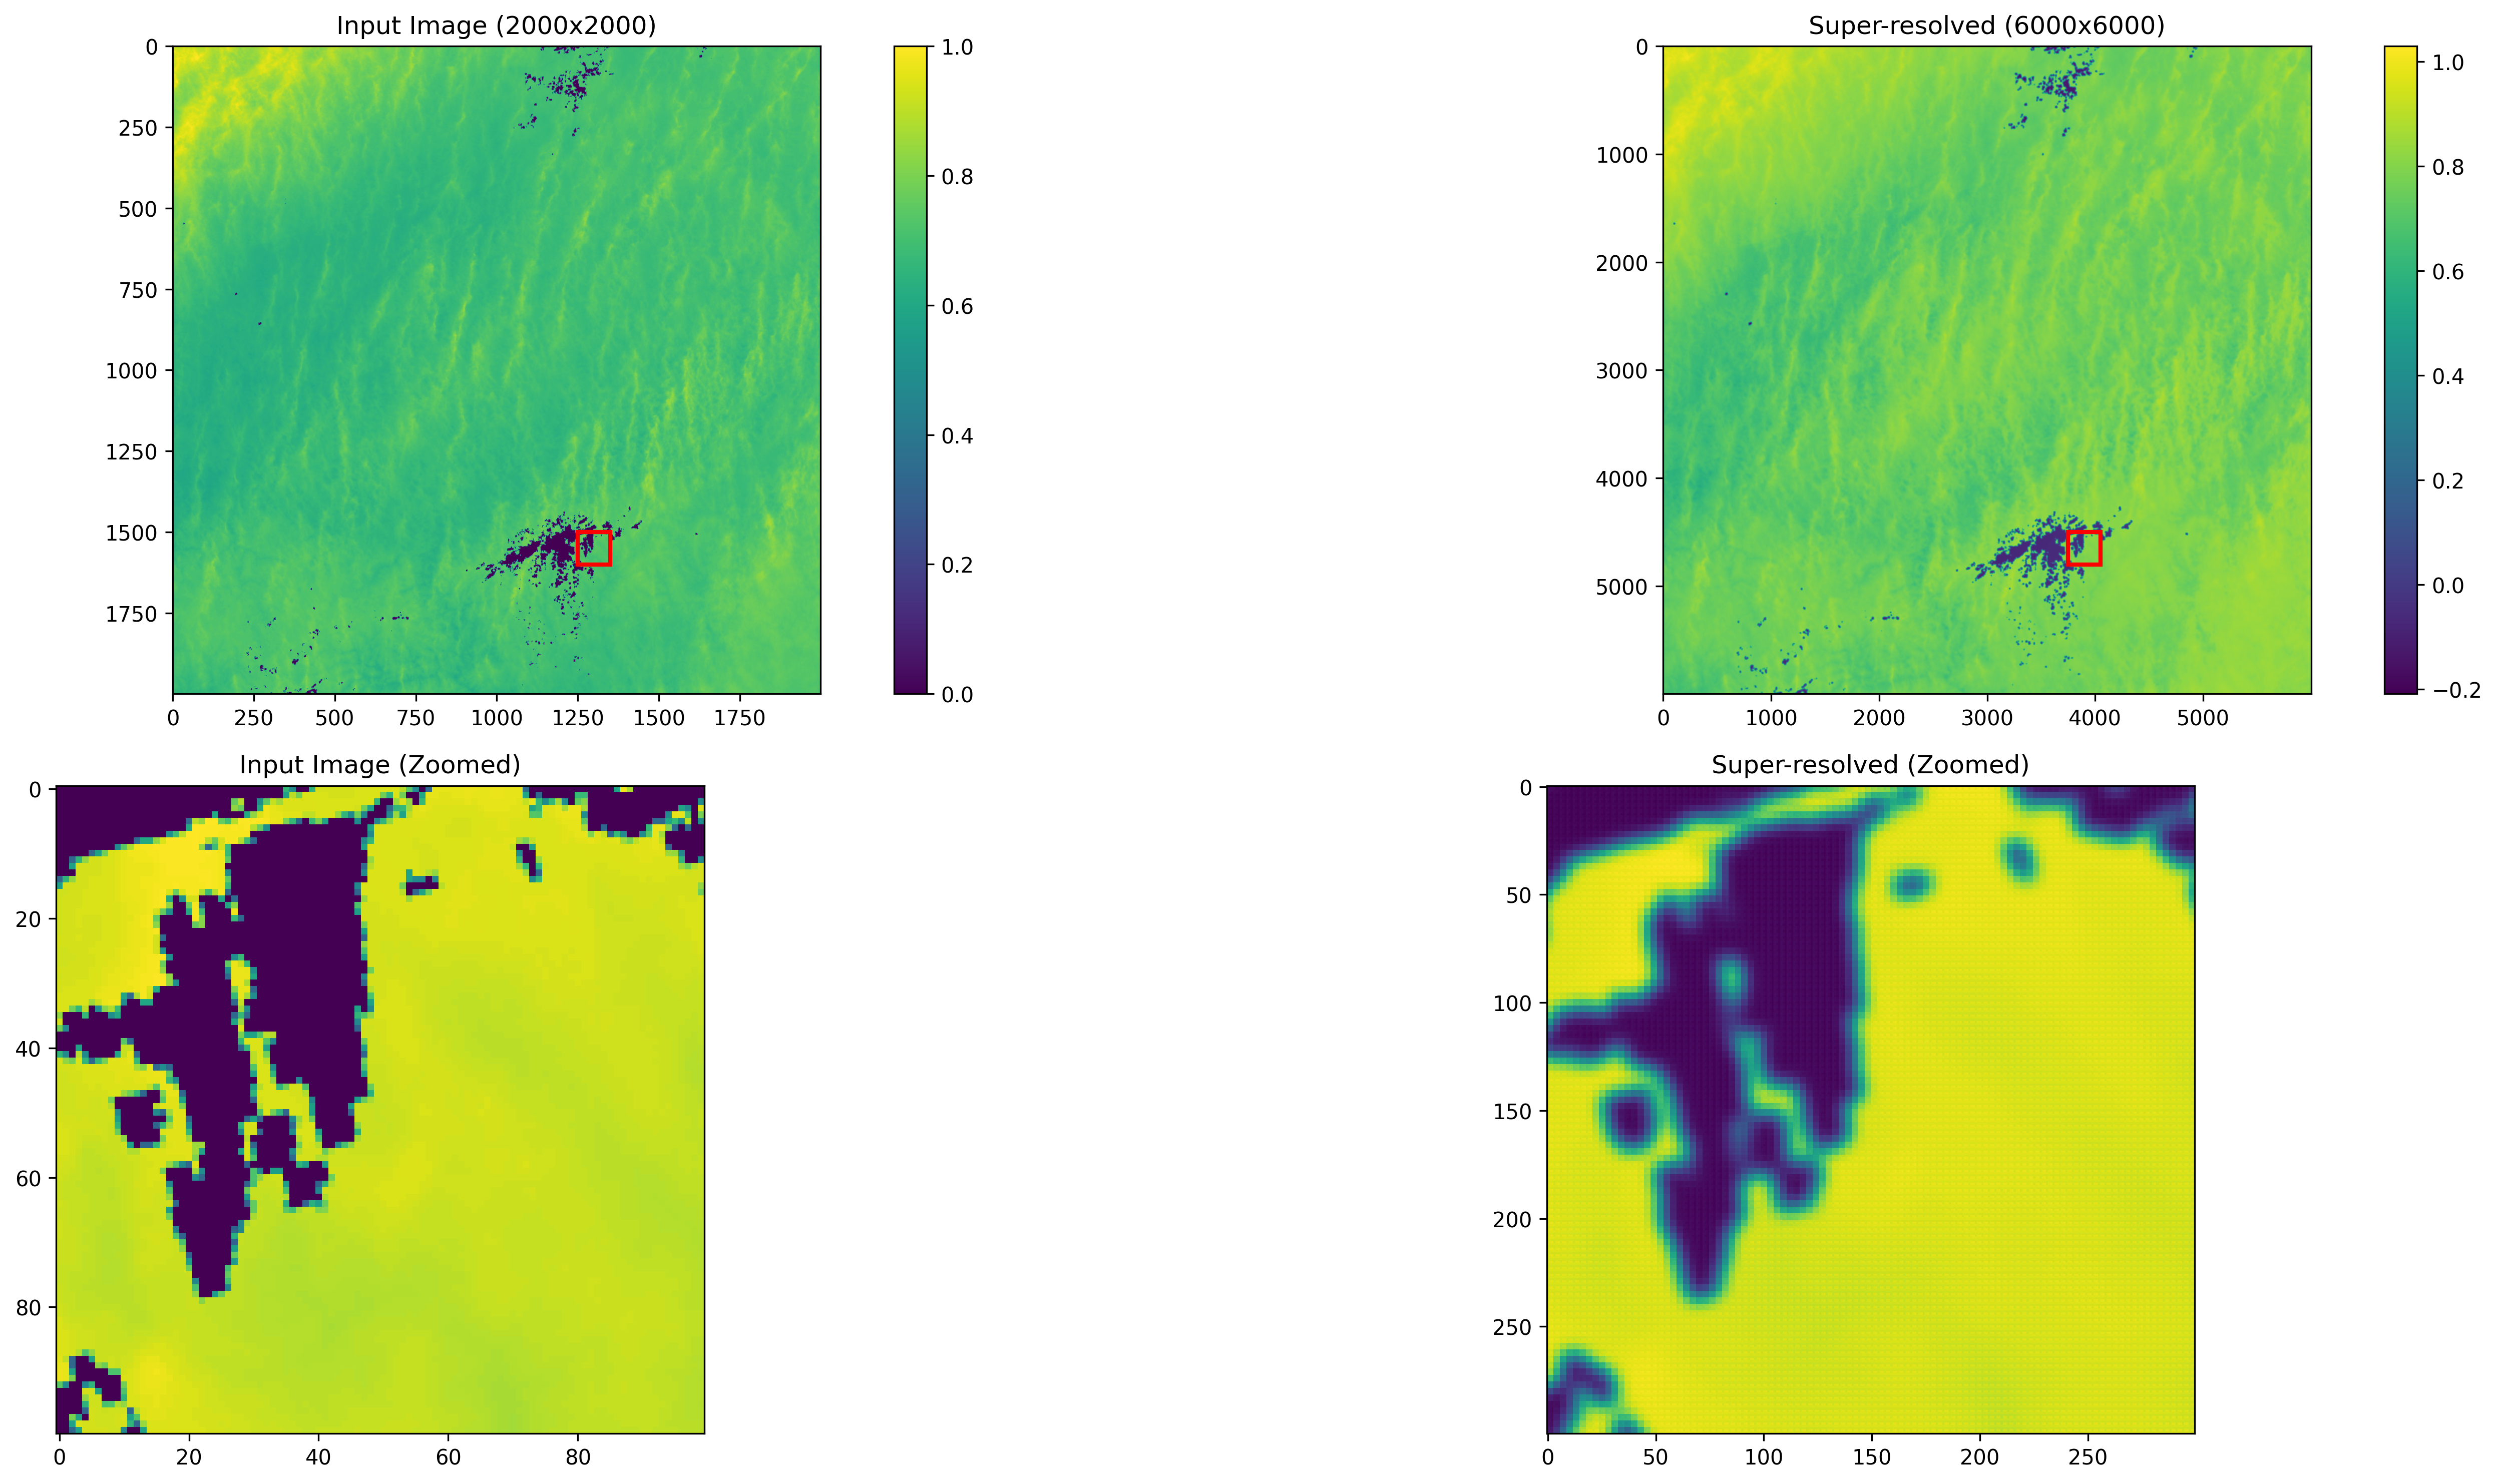
\includegraphics[width=\linewidth]{comparison_plot_with_zoom.png}
    \caption{Comparison of OG versus Upscaled image}
    \label{fig:comparison}
\end{figure}


\section{Convolutional Neural Network (CNN) - Alternative approach}

\subsection{Dataset Preparation}

For this model, we used Landsat 8 Band 10 images cropped to 3000x3000 pixels. To optimize memory usage, each image was divided into 40x40 zones of 75x75 pixels. Each 75x75 zone was then downscaled to 25x25 pixels by averaging 3x3 areas, resulting in one pixel. Unlike the previous approach, we did not rotate the images but instead cropped lines starting from each corner of the original photos. The final output images were cropped to 3000x3000 pixels.

\subsection{Model Architecture}

The CNN model was designed to take a 25x25 input region and output a 3x3 region, representing the zoomed-in center pixel. The architecture of the CNN includes multiple convolutional layers, followed by activation functions, designed to learn the features necessary for super-resolution. \subsection{Training Process}
The model was trained with a lr = 0.00001 and a batch size of 128 and 1 million epochs. Training was still done on temperature data, being converted from the pixel values of the band 10 images.
We employed two callbacks during training:
\begin{itemize} 
    \item **Early Stopping:** Training was stopped if the loss did not improve for 10 consecutive epochs.
    \item **Model Checkpoint:** The best model was saved whenever a new minimum loss was found.
\end{itemize}
The training ran for 176 epochs.

\begin{figure}[H]
    \centering
    \includegraphics[width=\linewidth]{cnn_loss_graph.png}
    \caption{Training Loss Over Time for CNN Model}
    \label{fig:cnnLossGraph}
\end{figure}

\subsection{Evaluation}
To assess the performance of the CNN model, we compared the original, low-resolution, and upscaled images. 
\begin{figure}[H]
    \centering
    \includegraphics[width=\linewidth]{cnn_comparison.png}
    \caption{Comparison of Original versus Output from the model}
    \label{fig:cnnComparison}
\end{figure}

The upscaled output is much clearer, and it seems to look better than the GCN model we used before. Training also took way less time using the new model, because of memory optimization. 

We obtained the following metrics after validation
\begin{itemize} 
    \item \textbf{Mean Squared Error (MSE):} 0.13340785437655 
    \item \textbf{Mean Absolute Error (MAE):} 0.0013708111975406 
    \item \textbf{R-squared (R2):} 0.954156922595998
\end{itemize}

In the end the CNN model was learning the patterns better (higher R2 score), and there was little error in the normalised data validation (values of the image pixels).





\chapter{Application (Study case)}
\label{chapter:application}


\section{App's description  and the main functionalities}
\label{section:appDescription}

We created a basic web application to for an easier usage of our developed model. We choose to utilise the second model (CNN) due to the better results and faster execution.


\section{App's design}
\label{section:appDesign}

The application is very simple, all the user needs to do is upload a satelite image (band 10, .TIF file) and press a button to see the resulted upscaled image (from 30m to 10m per pixel).

\section{Implementation}
\label{section:appImplementation}

The aplication uses a Flask server for the backend and vanilla js/html for the client side, but we are utilizing tiff.js for working with the satelite images. The backend is receiving the image and processing it using our trained model, then sending the result back to the client. The user can then download the resulting satelite image.



\chapter{Conclusion and future work}
\label{chapter:concl}

During our work, we created 2 models. The initial GNN (GCN) which was the main idea behind the problem, and the CNN. In the end, while the GCN was working, it had its limitations, such as same-size inputs, high memory cost (due to 8-neighbour connectivity for the graphs), and slow operation time. That is why we developed the second model, the CNN, which we optimized for memory (splitting the data in chunks), and we got even better results as shown previously! We believe a GCN might have the advantage in a better circumstance against a CNN, such as supercomputers with unlimited power and time, but for our use case the CNN was the way to go, and the results are super promising.




\bibliographystyle{plain}

\bibliography{BibAll}

\end{document}